\documentclass[12pt,a4j]{jreport}
\setcounter{secnumdepth}{5}
\usepackage[dvipdfmx]{graphicx}
\usepackage{amsmath,amssymb}
\usepackage{comment}
\usepackage{graphicx}
\usepackage{here}
\usepackage{bm}
\usepackage{url}

\renewcommand{\baselinestretch}{1.5}

\renewcommand{\bibname}{参考文献}





\begin{document}


%%%%%%%%%%%%%%%%%%%%%%%%%%%%%%%%%%%%%
% 表紙
%%%%%%%%%%%%%%%%%%%%%%%%%%%%%%%%%%%%%
\begin{titlepage}

\begin{center}

    \vspace*{2cm}
    \Large 2021 年度 芝浦工業大学 工学部 情報工学科\\

    \vspace*{1.0cm}
    \Huge 卒 \qquad 業 \qquad 論 \qquad 文\\
    \vspace*{2.5cm}

    %TODO 編集 : 題目
    \Large AAA及びBBBのための\\CCCを用いたDDDアルゴリズムに関する研究
    
    \vspace{4cm}
    \begin{tabular}{ll}
        %TODO 編集 : 題目
        \vspace*{2mm}
        学籍番号 & \qquad $\mathbf{AL18999}$ \\
        \vspace*{2mm}
        氏\phantom{  }名 & \qquad 芝浦 \quad 太郎   \\
        \vspace*{2mm}
        指導教員           & \qquad 〇〇 \quad 〇〇
    \end{tabular}
\end{center}
\end{titlepage}



\begin{abstract}
このファイルは,情報工学科卒業論文の推奨テンプレートである.概要書とは異なり,卒業論文本体のテンプレートはあくまで推奨であるので,このテンプレートを下にして文字サイズや行間などを修正したものを利用しても良く,またこのテンプレートを使わなくても良い.

この部分の研究概要では,研究背景,解決したい問題,研究目的,提案手法,評価方法,評価の結果について簡潔に書く.
概要の有無は任意.
\end{abstract}


{\makeatletter
\let\ps@jpl@in\ps@empty
\makeatother
\pagestyle{empty}
\tableofcontents
\clearpage}

\setcounter{page}{1} 
\pagestyle{plain}

%%%%%%%%%%%%%%%%%%%%%%%%%%%%%%%%%%%%%%%%%%%%%%%%%%%%%%%%%%%%%
% 序論 
%%%%%%%%%%%%%%%%%%%%%%%%%%%%%%%%%%%%%%%%%%%%%%%%%%%%%%%%%%%%%
\chapter{序論(この章タイトルは一例.各自内容に合わせてつけること)}

\section{背景}
このファイルは,情報工学科卒業論文の推奨テンプレートである.概要書とは異なり,卒業論文本体のテンプレートはあくまで推奨であるので,このテンプレートを下にして文字サイズや行間などを修正したものを利用しても良く,またこのテンプレートを使わなくても良い.


\subsection{図表参照の例,}
論文では,必要に応じて図や表を掲載し本文より参照すること.例えば,図の参照は『図\ref{fig_nn}に3層のニューラルネットワークを示す』,表の参照は『表\ref{table_a}に手法Aおよび手法Bの正答率を示す』などとする.図のキャプションは図の下に,表のキャプションは表の上に書く.

\begin{figure}[ht]
	\centering
	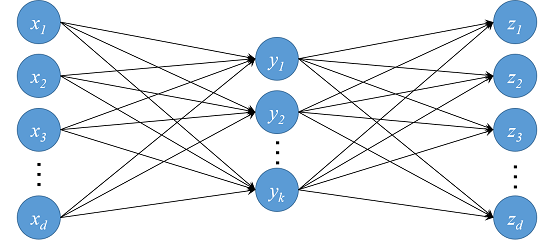
\includegraphics[keepaspectratio, width=120mm]{img/sample.png}
	\caption{提案法に用いた3層のニューラルネットワーク.キャプションにはこの図の説明を書く.}
	\label{fig_nn}
\end{figure}

\begin{table}[ht]
  \caption{手法Aおよび手法Bの正解率と平均計算時間.}
  \label{table_a}
  \centering
  \begin{tabular}{lcr}
    \hline
    手法   & 正解率[\%]  &  計算時間[ms]  \\
    \hline \hline
    手法A  & 92.3  & 512 \\
    手法B  & 87.4  & 32  \\
    \hline
  \end{tabular}
\end{table}



\subsection{関連研究参照の例}
参考文献は,『井尻らは,X線CTとデジタルカメラを用いた3次元モデリング法を提案した\cite{Ijiri18}.』のように引用する.参考文献リストは,『著者1, 著者2,...,著者N. タイトル. 論文誌or学会名, 巻, 号, ページ, 発表年. 』の形式とする.文献によっては,巻・号・ページがないものもある.
変化する可能性があるWebページの引用はあまり推奨されないが,Webページを引用する必要がある場合は末尾に参照日時を記入すること『著者. ページタイトル. ページURL(2021年7月31日参照).』参考文献リストについて,ref.bibファイルに引用したい文献情報を記載しておくと自動で整形されるので活用すると良い.


\section{Latexファイルのコンパイル方法}

\subsection{ローカルにLatex環境を構築する場合}
各自好みの環境を使ってコンパイルするとよい.例として,TeXLiveを利用す場合は以下の手順でpdfを構築できる.
(1) TexLive\cite{TexLive}をインストール.
(2) フォルダ内のresume.texをTexLiveと同梱されているTexWorksで開く.
(3) 左上で『pBibTex』を指定しコンパイルを実行.
(4) 左上で『pLatex』を指定しコンパイルを実行(参考文献が?となる場合はこれを複数回実行).


\subsection{Overleafを利用する場合}
Overleafを利用する場合,以下の手順でpdfを作成できる.
(1)フォルダ内のresume.tex, ref.bib, latexmkrc, img/sample.pngをoverleafのプロジェクトにコピー.
(2)OVerleafのメニューより,コンパイラを『LaTeX』に,TexLive versionを2020に変更.
(3)リコンパイルボタンを押す.
もしエラーが起こる場合,(*)右側の画面からキャッシュファイルを削除する,(*)コンパイラを違うものに変更してコンパイルしてから再度LaTeXでコンパイル,(*)フォルダをつくりその中でresume.texをコンパイル,などを試すとうまくいく場合がある.



\section{目的}



\section{本論文の構成}



%%%%%%%%%%%%%%%%%%%%%%%%%%%%%%%%%%%%%%%%%%%%%%%%%%%%%%%%%%%%%
%%%%%%%%%%%%%%%%%%%%%%%%%%%%%%%%%%%%%%%%%%%%%%%%%%%%%%%%%%%%%
\chapter{関連研究}

\section{グループ1}

\section{グループ2}




%%%%%%%%%%%%%%%%%%%%%%%%%%%%%%%%%%%%%%%%%%%%%%%%%%%%%%%%%%%%%
%%%%%%%%%%%%%%%%%%%%%%%%%%%%%%%%%%%%%%%%%%%%%%%%%%%%%%%%%%%%%
\chapter{提案手法}

\section{設計指針}

\section{システム構成}

\section{ユーザインタフェース}

\section{アルゴリズム}




%%%%%%%%%%%%%%%%%%%%%%%%%%%%%%%%%%%%%%%%%%%%%%%%%%%%%%%%%%%%%
%%%%%%%%%%%%%%%%%%%%%%%%%%%%%%%%%%%%%%%%%%%%%%%%%%%%%%%%%%%%%
\chapter{評価実験}


\section{仮説}
評価実験を設計するにあたり以下3件の仮説を立てる.
\begin{itemize}
  \item 仮説1) .
  \item 仮説2) 
  \item 仮説3) 
\end{itemize}
この3件の仮設は,それぞれ以下の考察に基づき設定されている.
仮説1は...


\section{実験手順}




%%%%%%%%%%%%%%%%%%%%%%%%%%%%%%%%%%%%%%%%%%%%%%%%%%%%%%%%%%%%%
%%%%%%%%%%%%%%%%%%%%%%%%%%%%%%%%%%%%%%%%%%%%%%%%%%%%%%%%%%%%%
\chapter{結果と考察}


\section{実験1について}


\section{実験2について}





%%%%%%%%%%%%%%%%%%%%%%%%%%%%%%%%%%%%%%%%%%%%%%%%%%%%%%%%%%%%%
%%%%%%%%%%%%%%%%%%%%%%%%%%%%%%%%%%%%%%%%%%%%%%%%%%%%%%%%%%%%%
\chapter{まとめと展望}





\chapter*{謝辞}
\addcontentsline{toc}{chapter}{謝辞}

\bibliographystyle{junsrt}
\bibliography{ref.bib}


\end{document}
